\chapter{Descrever um sistema químico: avanço, atividades, Q e K}\label{ch:b1:extent-q-and-k}

Uma unidade de produção de hidrogênio alimenta tubos aquecidos ao rubro
com gás natural e vapor d'água; o que sai nunca é hidrogênio puro, mas
uma mistura de hidrogênio, monóxido de carbono, dióxido de carbono,
metano não reagido e vapor, cujas proporções os engenheiros precisam
conhecer antes de projetar a unidade seguinte. Prever a composição que
sai de um reator --- o estado final de um sistema químico --- é o
assunto deste capítulo. Isso exige uma descrição precisa do sistema
(suas variáveis e sua composição), um único número que mede até onde
uma reação avançou (o avanço) e a lei que diz onde a reação para (a
constante de equilíbrio). Essas ferramentas são usadas em todos os
capítulos seguintes sobre as soluções.

\begin{recall}
O Livro 1 (ano 10) acompanhou uma reação com uma tabela de avanço e
encontrou o \omterm{def:b1:extent-q-and-k:max-extent}{reagente limitante}; o Livro 1 (ano 12) introduziu o
\omterm{def:b1:extent-q-and-k:quotient}{quociente de reação} $Q$ e a constante de equilíbrio $K$ de uma reação
não total. Da física, usamos a lei dos gases perfeitos $pV = nRT$, com $R =
\qty{8.314}{J/(mol.K)}$.
\end{recall}

\begin{omfigure}
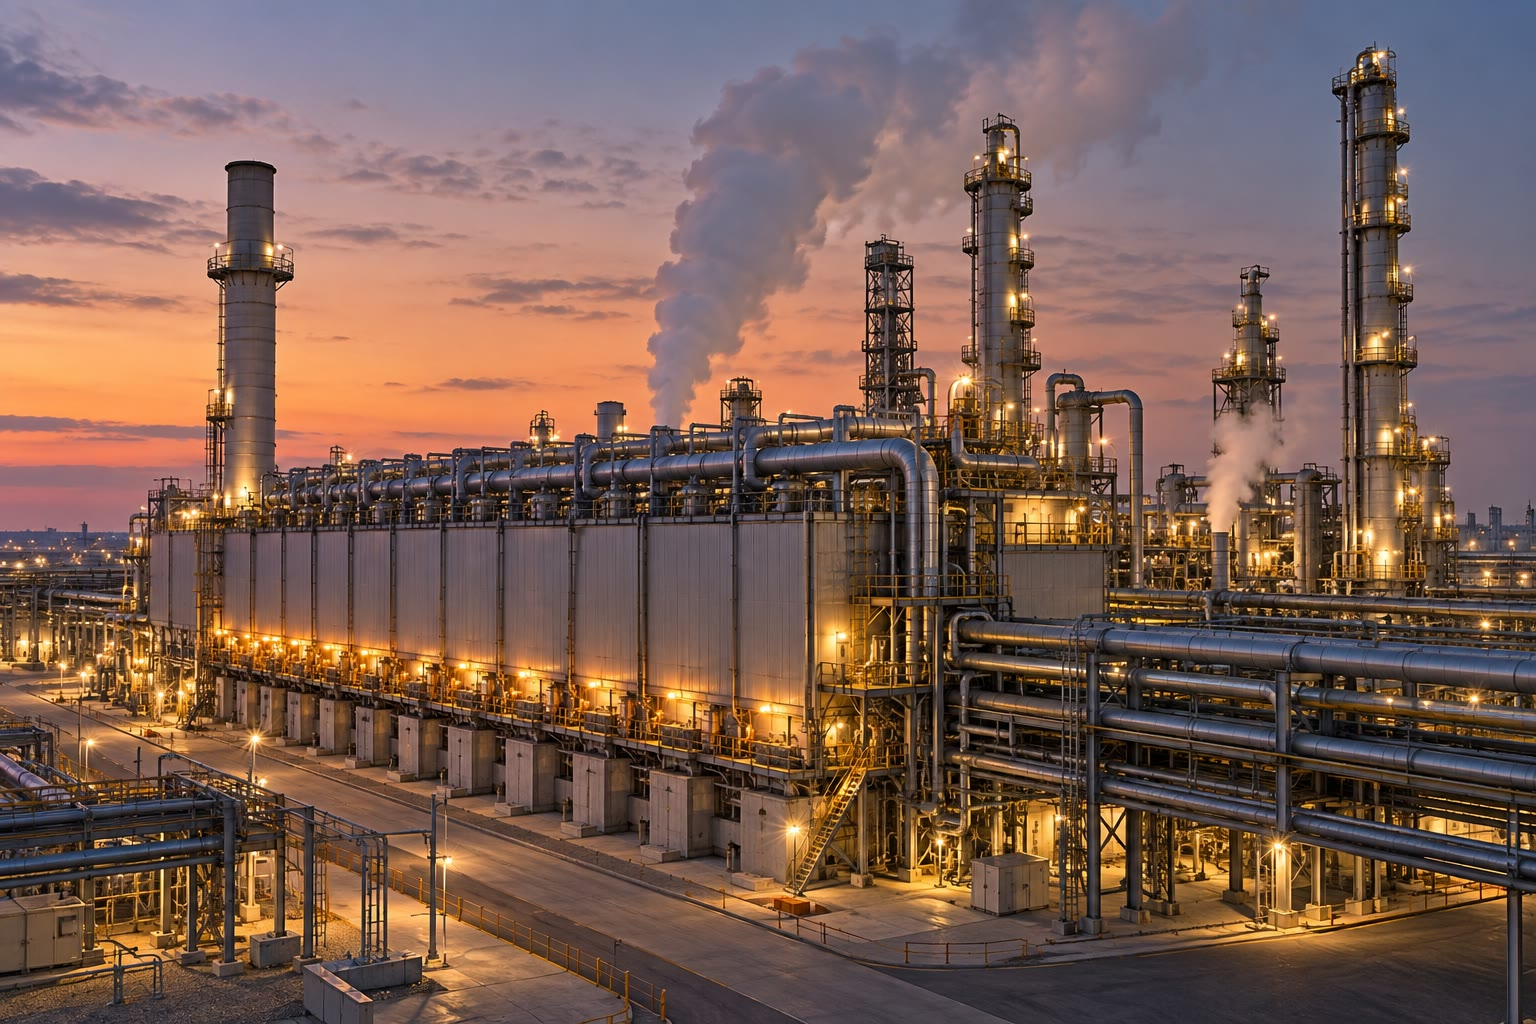
\includegraphics[width=0.6\linewidth]{images/book2/ai/b1-07-hydrogen-plant.jpg}

{\small Uma unidade de produção de hidrogênio ao entardecer. O gás
natural e o vapor reagem no longo forno de reforma; um segundo reator
converte o monóxido de carbono; a composição na saída é um estado final
do tipo calculado neste capítulo.}
\end{omfigure}

\section{Descrever um sistema}

\begin{definition}[Sistema, fase]\label{def:b1:extent-q-and-k:system}
Um \emph{sistema físico-químico}\index{sistema fisico-quimico@sistema físico-químico} é a
matéria contida em uma região do espaço escolhida, sendo o resto a sua
vizinhança. Ele é um \emph{sistema fechado}\index{sistema fechado} se não
troca matéria com a vizinhança (pode trocar energia). Uma
\emph{fase}\index{fase} é uma parte do sistema na qual as \omterm{def:b1:extent-q-and-k:variables}{variáveis
intensivas} variam continuamente: uma mistura gasosa é uma fase, dois
líquidos imiscíveis são duas fases, cada sólido é uma fase própria.
\end{definition}

\begin{definition}[Variáveis intensivas e extensivas]\label{def:b1:extent-q-and-k:variables}
Uma variável de estado é \emph{extensiva}\index{variavel extensiva@variável extensiva} se é
proporcional ao tamanho do sistema (massa, volume, quantidade de
matéria) e \emph{intensiva}\index{variavel intensiva@variável intensiva} se não é
(temperatura, pressão, concentração, massa específica, \omterm{def:b1:extent-q-and-k:composition}{fração molar}). A
razão entre duas variáveis extensivas é intensiva.
\end{definition}

\begin{definition}[Variáveis de composição]\label{def:b1:extent-q-and-k:composition}
Para um constituinte $i$ de uma \omterm{def:b1:extent-q-and-k:system}{fase} que contém as quantidades $n_j$ de
todos os seus constituintes:
\begin{itemize}
  \item sua \emph{fração molar}\index{fracao molar@fração molar} é $x_i = n_i/\sum_j
        n_j$, e sua \emph{fração mássica}\index{fracao massica@fração mássica} $w_i =
        m_i/\sum_j m_j$; ambas ficam entre 0 e 1 e somam 1;
  \item em uma solução de volume $V$, sua \emph{concentração
        molar}\index{concentracao molar@concentração molar} é $c_i = [i] = n_i/V$,
        em \unit{mol/L};
  \item em uma mistura gasosa sob pressão total $p$, sua \emph{pressão
        parcial}\index{pressao parcial@pressão parcial} é $p_i = x_i\,p$.
\end{itemize}
\end{definition}

\begin{proposition}[Pressões parciais dos gases perfeitos]\label{prop:b1:extent-q-and-k:dalton}
Em uma mistura de gases perfeitos de volume $V$ à temperatura $T$, a
\omterm{def:b1:extent-q-and-k:composition}{pressão parcial} de um constituinte é a pressão que ele exerceria sozinho
em todo o volume, $p_i = n_iRT/V$, e as \omterm{def:b1:extent-q-and-k:composition}{pressões parciais} somam a
pressão total: $\sum_i p_i = p$.
\end{proposition}

\begin{proof}
Para a mistura, $pV = (\sum_j n_j)RT$, logo $p_i = x_i p = \frac{n_i}{\sum_j
n_j}\cdot\frac{(\sum_j n_j)RT}{V} = \frac{n_iRT}{V}$, e $\sum_i x_i = 1$
dá $\sum_i p_i = p$.
\end{proof}

\begin{example}[O ar]\label{ex:b1:extent-q-and-k:air}
O ar seco contém, em volume (isto é, em quantidade de matéria, para
gases perfeitos), 78.08\,\% de dinitrogênio, 20.95\,\% de dioxigênio e
0.93\,\% de argônio. Sob \qty{1.013}{bar}, a \omterm{def:b1:extent-q-and-k:composition}{pressão parcial} do
dioxigênio é $0.2095 \times
1.013 = \qty{0.212}{bar}$; em uma montanha onde a pressão é de
\qty{0.70}{bar}, ela cai para \qty{0.147}{bar}, embora a composição seja
a mesma.
% ledger: air:N2, air:O2, air:Ar, const:atm
\end{example}

\section{Avanço da reação}

\begin{definition}[Números estequiométricos, avanço]\label{def:b1:extent-q-and-k:extent}
Uma reação é escrita $0 = \sum_i \nu_i\,\mathrm{A}_i$, em que o
\emph{número estequiométrico}\index{numero estequiometrico@número estequiométrico} $\nu_i$ da
espécie $\mathrm{A}_i$ é negativo para um reagente e positivo para um
produto: em \ce{N2 + 3H2 -> 2NH3}, $\nu(\ce{N2}) = -1$, $\nu(\ce{H2}) = -3$,
$\nu(\ce{NH3}) = +2$. Em um \omterm{def:b1:extent-q-and-k:system}{sistema fechado} em que só ocorre essa reação,
as quantidades variam segundo
\[
  n_i = n_{i,0} + \nu_i\,\xi ,
\]
o que define o \emph{avanço da reação}\index{avanco da reacao@avanço da reação}
$\xi$ (em mol), nulo no início e o mesmo para todas as espécies.
\end{definition}

\begin{definition}[Avanço máximo, reagente limitante]\label{def:b1:extent-q-and-k:max-extent}
O \emph{avanço máximo}\index{avanco maximo@avanço máximo} $\xi_{\max}$ é o maior
valor de $\xi$ para o qual nenhuma quantidade é negativa: $\xi_{\max} = \min_{\nu_i <
0} n_{i,0}/|\nu_i|$. O reagente que chega a zero em $\xi_{\max}$ é o
\emph{reagente limitante}\index{reagente limitante}. Quando o avanço
também pode ser negativo (reação inversa), $\xi_{\min} = -\min_{\nu_i > 0}
n_{i,0}/\nu_i$.
\end{definition}

\begin{method}[A tabela de avanço]\label{met:b1:extent-q-and-k:progress-table}
Para acompanhar uma reação em um \omterm{def:b1:extent-q-and-k:system}{sistema fechado}:
\begin{enumerate}
  \item escreva a equação balanceada e, abaixo dela, uma coluna por espécie;
  \item primeira linha: as quantidades iniciais $n_{i,0}$;
  \item segunda linha: as quantidades no avanço $\xi$, $n_{i,0} + \nu_i\xi$;
  \item para gases, acrescente uma coluna com a quantidade total $n_{\text{tot}}(\xi)$;
  \item calcule $\xi_{\max}$ (e $\xi_{\min}$) e identifique o \omterm{def:b1:extent-q-and-k:max-extent}{reagente
        limitante};
  \item última linha: as quantidades finais, no avanço final $\xi_f$
        (obtido pela condição de equilíbrio, ou igual a $\xi_{\max}$ se a
        reação for total).
\end{enumerate}
\end{method}

\begin{example}[Síntese da amônia]\label{ex:b1:extent-q-and-k:ammonia}
A partir de \qty{2.0}{mol} de \ce{N2} e \qty{3.0}{mol} de \ce{H2}:
\begin{center}
\begin{tabular}{lcccc}
\hline
 & \ce{N2} & \ce{3H2} & \ce{2NH3} & total \\
\hline
inicial & 2.0 & 3.0 & 0 & 5.0 \\
avanço $\xi$ & $2.0 - \xi$ & $3.0 - 3\xi$ & $2\xi$ & $5.0 - 2\xi$ \\
\hline
\end{tabular}
\end{center}
$\xi_{\max} = \min(2.0/1,\ 3.0/3) = \qty{1.0}{mol}$: o di-hidrogênio é o
limitante. Se a reação fosse total, o estado final conteria
\qty{1.0}{mol} de \ce{N2} e \qty{2.0}{mol} de \ce{NH3}.
\end{example}

\begin{definition}[Taxa de avanço final, rendimento]\label{def:b1:extent-q-and-k:fractional-extent}
A \emph{taxa de avanço final}\index{taxa de avanco final@taxa de avanço final} de uma
reação é $\tau = \xi_f/\xi_{\max}$, entre 0 e 1. Em uma síntese, o
\emph{rendimento}\index{rendimento} de um produto é a razão entre a
quantidade obtida e a quantidade que o \omterm{def:b1:extent-q-and-k:max-extent}{reagente limitante} daria se a
reação fosse total; quando o produto não é perdido durante o
isolamento, ele é igual a $\tau$.
\end{definition}

\section{Atividades}

\begin{definition}[Estado padrão, atividade]\label{def:b1:extent-q-and-k:activity}
A \emph{atividade}\index{atividade} $a_i$ de uma espécie é um número
adimensional que mede, na expressão das leis de equilíbrio, o quanto
dela está disponível; ela é definida em relação a um \emph{estado
padrão}\index{estado padrao@estado padrão}, um estado de referência à
temperatura considerada e sob a pressão padrão $p^\circ = \qty{1}{bar}$.
Nas aproximações ideais usadas neste livro:
\begin{itemize}
  \item para um gás, $a_i = p_i/p^\circ$ (o estado padrão é o gás
        perfeito puro a $p^\circ$);
  \item para um soluto em uma solução diluída, $a_i = c_i/c^\circ$ com
        $c^\circ = \qty{1}{mol/L}$;
  \item para o solvente de uma solução diluída, e para um sólido puro ou
        um líquido puro sozinho em sua \omterm{def:b1:extent-q-and-k:system}{fase}, $a_i = 1$.
\end{itemize}
\end{definition}
% ledger: const:pstd

\begin{remark}[Ideal e real]\label{rem:b1:extent-q-and-k:ideal}
Essas expressões valem para gases perfeitos e para soluções diluídas. Em
soluções concentradas, os íons se atraem e se repelem e a \omterm{def:b1:extent-q-and-k:activity}{atividade} se
afasta de $c_i/c^\circ$; as correções, escritas com coeficientes de
\omterm{def:b1:extent-q-and-k:activity}{atividade}, são estudadas no volume do 2.º ano com o potencial químico.
Para as concentrações usadas neste livro (abaixo de cerca de
\qty{0.1}{mol/L}), as expressões ideais são exatas a alguns por cento.
\end{remark}

\section{O quociente de reação e a constante de equilíbrio}

\begin{definition}[Quociente de reação]\label{def:b1:extent-q-and-k:quotient}
O \emph{quociente de reação}\index{quociente de reacao@quociente de reação} de uma reação
$0 = \sum_i \nu_i\,\mathrm{A}_i$ em um dado estado do sistema é
\[
  Q = \prod_i a_i^{\nu_i} ,
\]
o produto das \omterm{def:b1:extent-q-and-k:activity}{atividades} dos produtos dividido pelo dos reagentes, cada
uma elevada à potência de seu coeficiente estequiométrico.
\end{definition}

\begin{example}[Três quocientes]\label{ex:b1:extent-q-and-k:quotients}
Para \ce{N2(g) + 3H2(g) <=> 2NH3(g)}: $Q = \dfrac{(p_{\ce{NH3}}/p^\circ)^2}
{(p_{\ce{N2}}/p^\circ)(p_{\ce{H2}}/p^\circ)^3}$. Para
\ce{CH3COOH(aq) + H2O(l) <=> CH3COO^-(aq) + H3O+(aq)}: $Q =
\dfrac{[\ce{CH3COO-}][\ce{H3O+}]}{[\ce{CH3COOH}]\,c^\circ}$, pois o
solvente tem \omterm{def:b1:extent-q-and-k:activity}{atividade} 1. Para \ce{CaCO3(s) <=> CaO(s) + CO2(g)}: $Q =
p_{\ce{CO2}}/p^\circ$, pois os sólidos têm \omterm{def:b1:extent-q-and-k:activity}{atividade} 1.
\end{example}

\begin{definition}[Constante de equilíbrio padrão]\label{def:b1:extent-q-and-k:equilibrium-constant}
A \emph{constante de equilíbrio padrão}\index{constante de equilibrio padrao@constante de equilíbrio padrão}
$K^\circ$ de uma reação é o valor que seu \omterm{def:b1:extent-q-and-k:quotient}{quociente de reação} assume
quando o sistema está em equilíbrio. Ela é adimensional e depende apenas
da reação e da temperatura.
\end{definition}

\begin{theorem}[Lei da ação das massas]\label{thm:b1:extent-q-and-k:mass-action}
A uma temperatura dada, um sistema em que uma reação pode ocorrer nos
dois sentidos evolui até que $Q = K^\circ(T)$; no equilíbrio, qualquer
que seja a composição inicial,
\[
  \prod_i a_{i,\text{eq}}^{\nu_i} = K^\circ(T) .
\]
\end{theorem}
\admitted

\begin{proposition}[Sentido de evolução]\label{prop:b1:extent-q-and-k:direction}
Um sistema em que $Q < K^\circ$ evolui no sentido direto ($\xi$
aumenta); se $Q > K^\circ$, evolui no sentido inverso; se
$Q = K^\circ$, está em equilíbrio.
\end{proposition}
\admitted

\begin{remark}[De onde vêm essas leis]\label{rem:b1:extent-q-and-k:origin}
Os dois enunciados decorrem do segundo princípio da termodinâmica, por
meio da energia livre de reação e dos potenciais químicos das espécies:
eles são deduzidos no volume do 2.º ano, que também obtém $K^\circ$ a
partir de tabelas de dados termodinâmicos e explica como ela varia com a
temperatura. Aqui, eles são usados como leis.
\end{remark}

\begin{omfigure}
\begin{tikzpicture}[font=\small, >={Stealth}]
  \draw[->, thick] (0,0) -- (11,0) node[right] {$Q$};
  \draw[thick, omThm] (5.5,0.25) -- (5.5,-0.25) node[below] {$K^\circ$};
  \draw[->, omDef, thick] (1.0,0.55) -- (4.6,0.55);
  \node[above, omDef] at (2.8,0.6) {$Q < K^\circ$: sentido direto};
  \draw[->, omProp, thick] (10.0,0.55) -- (6.4,0.55);
  \node[above, omProp] at (8.2,0.6) {$Q > K^\circ$: sentido inverso};
  \node[below] at (0,-0.1) {0};
\end{tikzpicture}

{\small O quociente se move em direção à constante: um sistema com $Q <
K^\circ$ forma produtos; um sistema com $Q > K^\circ$ os consome.}
\end{omfigure}

\begin{proposition}[Combinação de constantes]\label{prop:b1:extent-q-and-k:combine-k}
Se $K_1^\circ$ e $K_2^\circ$ são as constantes das reações (1) e (2):
a inversa de (1) tem a constante $1/K_1^\circ$; a reação $n \times
(1)$ tem $(K_1^\circ)^n$; a soma $(1) + (2)$ tem $K_1^\circ K_2^\circ$.
\end{proposition}

\begin{proof}
O quociente da reação inversa é $\prod a_i^{-\nu_i} = 1/Q_1$; o de
$n \times (1)$ é $\prod a_i^{n\nu_i} = Q_1^n$; o da soma é
$\prod a_i^{\nu_{i,1} + \nu_{i,2}} = Q_1 Q_2$. Escrevendo essas
identidades no equilíbrio, em que cada quociente é igual a sua
constante, obtém-se o resultado.
\end{proof}

\begin{proposition}[Um único estado de equilíbrio]\label{prop:b1:extent-q-and-k:q-monotone}
Para uma única reação em um \omterm{def:b1:extent-q-and-k:system}{sistema fechado} a temperatura fixa (e, para
gases, a volume ou pressão fixos), o quociente $Q(\xi)$ é uma função
estritamente crescente de $\xi$ em $(\xi_{\min}, \xi_{\max})$, que vai de 0
a $+\infty$ quando não há espécie de \omterm{def:b1:extent-q-and-k:activity}{atividade} constante envolvida. A
equação $Q(\xi) = K^\circ$ tem então exatamente uma solução nesse
intervalo.
\end{proposition}

\begin{proof}
Considere uma reação em solução, $Q(\xi) = \prod_i (n_{i,0} + \nu_i\xi)^{\nu_i}
\times \text{cte}$. Sua derivada logarítmica é
\[
  \frac{\dd \ln Q}{\dd \xi} = \sum_i \frac{\nu_i^2}{n_{i,0} + \nu_i \xi}
  > 0 ,
\]
cada termo sendo positivo onde todas as quantidades o são. Quando
$\xi \to \xi_{\max}$, a quantidade de um reagente tende a 0 em um
denominador e $Q \to +\infty$; quando $\xi
\to \xi_{\min}$, a quantidade de um produto tende a 0 e $Q \to 0$. Uma
função contínua e crescente de 0 a $+\infty$ assume o valor $K^\circ$
uma única vez. (Para gases a pressão constante, a quantidade total também
varia; o resultado continua valendo, como se pode verificar em cada
caso.)
\end{proof}

\section{Estados finais}

\begin{definition}[Estado de equilíbrio, reação quantitativa]\label{def:b1:extent-q-and-k:quantitative}
O estado final é um \emph{estado de equilíbrio}\index{estado de equilibrio@estado de equilíbrio}
quando todas as espécies da reação estão presentes e $Q = K^\circ$. A
reação é \emph{quantitativa}\index{reacao quantitativa@reação quantitativa} (ou total)
quando, no estado final, o \omterm{def:b1:extent-q-and-k:max-extent}{reagente limitante} praticamente desapareceu,
$\xi_f \approx \xi_{\max}$; isso acontece quando $K^\circ$ é muito
grande.
\end{definition}

\begin{method}[Encontrar o estado final]\label{met:b1:extent-q-and-k:final-state}
Para encontrar o estado final de uma única reação:
\begin{enumerate}
  \item monte a tabela de avanço e calcule $\xi_{\max}$ (e $\xi_{\min}$);
  \item calcule $Q$ no início e compare-o com $K^\circ$ para encontrar o
        sentido;
  \item expresse $Q(\xi)$ com as \omterm{def:b1:extent-q-and-k:activity}{atividades} e resolva $Q(\xi) = K^\circ$
        para $\xi$ em $(\xi_{\min}, \xi_{\max})$;
  \item se uma espécie de \omterm{def:b1:extent-q-and-k:activity}{atividade} 1 (um sólido) estiver envolvida,
        verifique se ela ainda está presente nesse avanço: se ela tivesse
        de ficar negativa, desaparece antes e o estado final \emph{não} é
        um equilíbrio ($\xi_f = \xi_{\max}$, $Q_f \ne K^\circ$).
\end{enumerate}
\end{method}

\begin{method}[A hipótese de reação quantitativa]\label{met:b1:extent-q-and-k:quantitative}
Quando $K^\circ$ é grande (tipicamente acima de $10^4$), suponha a
reação total: tome $\xi_f = \xi_{\max}$, calcule as quantidades finais e
depois encontre a pequena quantidade $\varepsilon$ de \omterm{def:b1:extent-q-and-k:max-extent}{reagente limitante}
restante escrevendo $Q =
K^\circ$ com as outras quantidades inalteradas. A hipótese é aceita se
$\varepsilon$ for pequena diante das outras quantidades (abaixo de cerca
de 1\,\%).
\end{method}

\begin{example}[Uma reação quantitativa]\label{ex:b1:extent-q-and-k:quant}
Para $\mathrm{A + B \rightleftharpoons C + D}$ em solução com $[\ce{A}]_0 = [\ce{B}]_0 =
\qty{0.10}{mol/L}$ e $K^\circ = 10^6$: supondo a reação total, $[\ce{C}]
= [\ce{D}] = 0.10$; então $0.10^2/\varepsilon^2 = 10^6$ dá $\varepsilon
= \qty{1.0e-4}{mol/L}$, 0.1\,\% da quantidade inicial: a hipótese se
justifica.
\end{example}

\begin{omfigure}
\begin{tikzpicture}
\begin{axis}[
  width=0.45\linewidth, height=5.6cm, ymode=log,
  xmin=0, xmax=1, ymin=0.01, ymax=1000,
  axis x line=bottom, axis y line=left,
  xlabel={avanço $\xi$ (mol)}, ylabel={$Q$}, xtick={0,0.2,0.4,0.8,1},
  tick label style={font=\small}, label style={font=\small}, clip=false]
\addplot[omDef, thick] table[x=xi, y=Q] {figdata/out/bachelor-1-extent-equilibrium-shift.dat};
\draw[omThm, dashed] (axis cs:0,4) -- (axis cs:1,4);
\node[omThm, anchor=south west, font=\small] at (axis cs:0.02,4) {$K^\circ = 4.0$};
\draw[dotted] (axis cs:0.607,0.01) -- (axis cs:0.607,4);
\node[anchor=north, font=\small] at (axis cs:0.607,0.01) {0.607};
\end{axis}
\end{tikzpicture}\hfill
\begin{tikzpicture}
\begin{axis}[
  width=0.45\linewidth, height=5.6cm,
  xmin=0, xmax=0.04, ymin=0, ymax=0.3,
  axis x line=bottom, axis y line=left,
  xlabel={avanço $\xi$ (mol)}, ylabel={$Q = p_{\ce{CO2}}/p^\circ$},
  xtick={0,0.01,0.02,0.03,0.04}, scaled x ticks=false,
  xticklabel style={/pgf/number format/fixed, /pgf/number format/precision=2},
  yticklabel style={/pgf/number format/fixed},
  tick label style={font=\small}, label style={font=\small}, clip=false]
\addplot[omProp, thick] table[x=xi, y=Q_small] {figdata/out/bachelor-1-extent-equilibrium-carbonate.dat};
\addplot[omDef, thick, dashed] table[x=xi, y=Q_large] {figdata/out/bachelor-1-extent-equilibrium-carbonate.dat};
\draw[omThm, dashed] (axis cs:0,0.2) -- (axis cs:0.04,0.2);
\node[omThm, anchor=south west, font=\small] at (axis cs:0.0005,0.2) {$K^\circ = 0.20$};
\node[omProp, anchor=north west, font=\scriptsize] at (axis cs:0.012,0.088) {\qty{0.010}{mol}: sólido esgotado};
\node[omDef, anchor=north west, font=\scriptsize] at (axis cs:0.024,0.19) {\qty{0.050}{mol}: equilíbrio};
\end{axis}
\end{tikzpicture}

{\small À esquerda: o quociente de \ce{CO + H2O <=> CO2 + H2} cresce com
o avanço e encontra $K^\circ$ uma única vez (problema de fim de semana).
À direita: para \ce{CaCO3(s) <=> CaO(s) + CO2(g)} em um recipiente
fechado de \qty{10}{L}, $Q = p_{\ce{CO2}}/p^\circ$ cresce com $\xi$; com
\qty{0.050}{mol} de carbonato, ele atinge $K^\circ = 0.20$ (equilíbrio);
com \qty{0.010}{mol}, o carbonato se esgota antes e o estado final não é
um equilíbrio.}
\end{omfigure}

\begin{method}[Duas reações simultâneas]\label{met:b1:extent-q-and-k:two-reactions}
Quando duas reações ocorrem no mesmo sistema, dê a cada uma seu próprio
avanço, $\xi_1$ e $\xi_2$; cada quantidade é $n_i = n_{i,0} + \nu_{i,1}\xi_1
+ \nu_{i,2}\xi_2$, e o estado final satisfaz $Q_1 = K_1^\circ$ e
$Q_2 = K_2^\circ$ (um sistema de duas equações). Se uma constante for
muito maior que a outra, trate primeiro a reação correspondente como
\omterm{def:b1:extent-q-and-k:quantitative}{quantitativa} e depois a segunda a partir do resultado.
\end{method}

\begin{history}[A lei da ação das massas, 1864]
Em 1864, o químico norueguês Cato Guldberg e seu cunhado, o farmacêutico
Peter Waage, publicaram em norueguês sua lei das ``massas ativas'': uma
reação avança até que as forças das reações direta e inversa se
equilibrem, cada uma proporcional às concentrações de seus reagentes. O
trabalho deles passou despercebido no exterior até que o republicassem
em duas línguas mais lidas, em 1867 e 1879; Jacobus van 't Hoff, que
havia redescoberto a lei, reconheceu a prioridade deles.
\end{history}

\section{Exercícios}

\begin{exercise}[$\star$]\label{exo:b1:extent-q-and-k:1}
Classifique como \omterm{def:b1:extent-q-and-k:variables}{intensiva} ou \omterm{def:b1:extent-q-and-k:variables}{extensiva}: temperatura, volume, quantidade
de matéria, \omterm{def:b1:extent-q-and-k:composition}{concentração molar}, massa específica, pressão, massa, \omterm{def:b1:extent-q-and-k:composition}{fração
molar}.
\end{exercise}

\begin{exercise}[$\star$]\label{exo:b1:extent-q-and-k:2}
Usando a composição do ar seco dada no capítulo, calcule as \omterm{def:b1:extent-q-and-k:composition}{pressões
parciais} de \ce{N2}, \ce{O2} e \ce{Ar} sob uma pressão total de
\qty{1.013}{bar}.
\end{exercise}

\begin{exercise}[$\star$]\label{exo:b1:extent-q-and-k:3}
Monte a tabela de avanço de \ce{2H2 + O2 -> 2H2O} a partir de
\qty{3.0}{mol} de \ce{H2} e \qty{2.0}{mol} de \ce{O2}. Encontre
$\xi_{\max}$, o \omterm{def:b1:extent-q-and-k:max-extent}{reagente limitante} e o estado final, se a reação for total.
\end{exercise}

\begin{exercise}[$\star$]\label{exo:b1:extent-q-and-k:4}
Escreva o \omterm{def:b1:extent-q-and-k:quotient}{quociente de reação} de: (a) \ce{CaCO3(s) <=> CaO(s) + CO2(g)};
(b) \ce{Ag+(aq) + Cl-(aq) <=> AgCl(s)}; (c) \ce{N2(g) + 3H2(g) <=>
2NH3(g)}; (d) \ce{NH3(aq) + H2O(l) <=> NH4+(aq) + OH-(aq)}.
\end{exercise}

\begin{exercise}[$\star\star$]\label{exo:b1:extent-q-and-k:5}
As reações (1) $\mathrm{A \rightleftharpoons B}$ e (2) $\mathrm{B \rightleftharpoons C}$ têm as constantes
$K_1^\circ = 10$ e $K_2^\circ = 0.5$. Dê as constantes de $\mathrm{A \rightleftharpoons C}$,
$\mathrm{C \rightleftharpoons A}$ e $\mathrm{2\,A \rightleftharpoons 2\,C}$.
\end{exercise}

\begin{exercise}[$\star\star$]\label{exo:b1:extent-q-and-k:6}
Uma reação tem $K^\circ = 2.0 \times 10^{-3}$. Em que sentido o sistema
evolui se, no início, $Q = 5.0 \times 10^{-5}$? E se $Q = 0.10$?
E se só houver reagentes?
\end{exercise}

\begin{exercise}[$\star\star$]\label{exo:b1:extent-q-and-k:7}
O gás \ce{A2} se dissocia, \ce{A2(g) <=> 2A(g)}, com $K^\circ = 0.25$ à
temperatura do experimento. Partindo de \qty{1.0}{mol} de \ce{A2} sob
uma pressão total mantida igual a $p^\circ$, monte a tabela de avanço
com a quantidade total, expresse $Q(\xi)$ e encontre o avanço de
equilíbrio.
\end{exercise}

\begin{exercise}[$\star\star$]\label{exo:b1:extent-q-and-k:8}
Em solução, $\mathrm{A + B \rightleftharpoons C}$ com $K^\circ = 100$ e concentrações
iniciais $[\ce{A}]_0 = [\ce{B}]_0 = \qty{0.10}{mol/L}$. Encontre as
concentrações de equilíbrio e a \omterm{def:b1:extent-q-and-k:fractional-extent}{taxa de avanço final}.
\end{exercise}

\begin{exercise}[$\star\star$]\label{exo:b1:extent-q-and-k:9}
Para $\mathrm{A + B \rightleftharpoons C + D}$ a partir de quantidades iguais de \ce{A} e \ce{B}, mostre que
a \omterm{def:b1:extent-q-and-k:fractional-extent}{taxa de avanço final} é $\tau = \sqrt{K^\circ}/(1 + \sqrt{K^\circ})$.
Que valor de $K^\circ$ dá $\tau = 0.99$?
\end{exercise}

\begin{exercise}[$\star\star\star$]\label{exo:b1:extent-q-and-k:10}
O carbonato de cálcio é aquecido a \qty{1100}{K} em um recipiente
fechado de \qty{10.0}{L}, inicialmente sem gás, para o qual
$K^\circ = 0.20$ para \ce{CaCO3(s) <=> CaO(s) + CO2(g)}. Encontre o
estado final para \qty{0.010}{mol} e para \qty{0.050}{mol} de carbonato.
\end{exercise}

\begin{exercise}[$\star\star\star$]\label{exo:b1:extent-q-and-k:11}
Uma substância \ce{A} se isomeriza em solução de duas maneiras, $\mathrm{A \rightleftharpoons B}$
($K_1^\circ = 2.0$) e $\mathrm{A \rightleftharpoons C}$ ($K_2^\circ = 3.0$). Partindo de
\qty{1.0}{mol} de \ce{A} sozinho, encontre as quantidades finais dos três
isômeros.
\end{exercise}

\begin{exercise}[$\star\star\star$]\label{exo:b1:extent-q-and-k:12}
Um ácido \ce{A} e um álcool \ce{B} dão um éster e água, $\mathrm{A + B
\rightleftharpoons E + W}$, tudo em uma única \omterm{def:b1:extent-q-and-k:system}{fase} líquida, com $K^\circ = 4.0$ (tome
as \omterm{def:b1:extent-q-and-k:activity}{atividades} iguais às \omterm{def:b1:extent-q-and-k:composition}{frações molares}; a quantidade total não varia).
Calcule o \omterm{def:b1:extent-q-and-k:fractional-extent}{rendimento} máximo em éster a partir de \qty{0.50}{mol} de cada
reagente e, depois, a partir de \qty{0.50}{mol} de ácido e \qty{1.0}{mol}
de álcool.
\end{exercise}

\section{Problema: A saída de uma unidade de hidrogênio}

\begin{problem}[{Problema de fim de semana --- as variáveis de composição
de uma alimentação, a reforma a vapor tratada como total, a reação de
deslocamento gás-água em equilíbrio e o teor de hidrogênio do gás que
sai da unidade}]
\label{pb:b1:extent-q-and-k:1}
Uma unidade de produção de hidrogênio é alimentada com \qty{1.00}{mol} de
metano e \qty{3.00}{mol} de vapor d'água (por unidade de tempo) sob
\qty{30}{bar}. No reformador, \ce{CH4 + H2O -> CO + 3H2} é suposta
total. No reator de deslocamento, \ce{CO + H2O <=> CO2 + H2} atinge o
equilíbrio; considere $K^\circ =
4.0$ à sua temperatura. Massas molares: \ce{CH4} \qty{16.04}{g/mol},
\ce{H2O} \qty{18.02}{g/mol}.

\medskip
\noindent\textbf{Parte I --- A alimentação.}
\begin{enumerate}
  \item Calcule as \omterm{def:b1:extent-q-and-k:composition}{frações molares} do metano e do vapor na alimentação.
  \item Calcule suas \omterm{def:b1:extent-q-and-k:composition}{pressões parciais}.
  \item Calcule suas \omterm{def:b1:extent-q-and-k:composition}{frações mássicas}.
  \item Quais das grandezas usadas até aqui são \omterm{def:b1:extent-q-and-k:variables}{intensivas}?
  \item Dê as \omterm{def:b1:extent-q-and-k:activity}{atividades} do metano e do vapor na alimentação.
\end{enumerate}

\medskip
\noindent\textbf{Parte II --- A reforma.}
\begin{enumerate}[resume]
  \item Monte a tabela de \omterm{def:b1:extent-q-and-k:extent}{avanço da reação} de reforma.
  \item Calcule $\xi_{\max}$ e indique o \omterm{def:b1:extent-q-and-k:max-extent}{reagente limitante}.
  \item Dê as quantidades que saem do reformador.
  \item Calcule a quantidade total de gás e compare-a com a da alimentação.
  \item Calcule as \omterm{def:b1:extent-q-and-k:composition}{frações molares} na saída do reformador.
  \item Por que o vapor é alimentado em excesso?
\end{enumerate}

\medskip
\noindent\textbf{Parte III --- O reator de deslocamento.}
\begin{enumerate}[resume]
  \item Monte a tabela de \omterm{def:b1:extent-q-and-k:extent}{avanço da reação} de deslocamento, partindo do
        gás que sai do reformador.
  \item Mostre que $Q(\xi) = \dfrac{\xi(3 + \xi)}{(1 - \xi)(2 - \xi)}$ e
        que ele não depende da pressão.
  \item Calcule $Q$ na entrada e preveja o sentido de evolução.
  \item Escreva a equação do avanço de equilíbrio e resolva-a,
        conservando a raiz que faz sentido.
  \item Dê as quantidades que saem do reator de deslocamento.
  \item Calcule a \omterm{def:b1:extent-q-and-k:fractional-extent}{taxa de avanço final} da reação de deslocamento.
  \item Com o dobro de vapor na alimentação (\qty{6.00}{mol}), o gás
        entra no reator de deslocamento com \qty{5.00}{mol} de vapor:
        calcule o novo avanço de equilíbrio.
\end{enumerate}

\medskip
\noindent\textbf{Parte IV --- O que sai da unidade.}
\begin{enumerate}[resume]
  \item Que valor de $K^\circ$ seria necessário para converter 99\,\% do
        monóxido de carbono no primeiro caso?
  \item Explique por que um reator de deslocamento converte mais quando
        opera a uma temperatura em que sua constante é maior, e por que
        as unidades usam dois reatores de deslocamento em série.
  \item O vapor é condensado do gás que sai do reator de deslocamento.
        Calcule a \omterm{def:b1:extent-q-and-k:composition}{fração molar} de hidrogênio no gás seco.
  \item Liste as impurezas que restam e suas quantidades.
  \item Calcule a \omterm{def:b1:extent-q-and-k:composition}{fração molar} de hidrogênio no gás que sai do reator de
        deslocamento, incluindo o vapor.
\end{enumerate}
\end{problem}
